%%%%%%%%%%%%%%%%%%%%%%%%%%%%%%%%%%%%%%%%%%%%%%%%%%%%%%%%%%%%%%%%%%%%%%%%%%%%%%%%%%%%
% Document data
%%%%%%%%%%%%%%%%%%%%%%%%%%%%%%%%%%%%%%%%%%%%%%%%%%%%%%%%%%%%%%%%%%%%%%%%%%%%%%%%%%%%
\documentclass[12pt]{article} %report allows for chapters
%%%%%%%%%%%%%%%%%%%%%%%%%%%%%%%%%%%%%%%%%%%%%%%%%%%%%%%%%%%%%%%%%%%%%%%%%%%%%%%%%%%%
\usepackage{preamble}
\usepackage{hyperref}

\begin{document}

\begin{center}
   \textsc{\large MATH 271, Worksheet 2, \emph{Solutions}}\\
   \textsc{Ordinary Differential Equations}
\end{center}
\vspace{.5cm}

\begin{center}
    Problems 1-6 are related.
\end{center}

\begin{problem}
    (Newton's law of cooling) Write down a differential equation that models the following scenario:\\
    
    \noindent\emph{The temperature of a substance in an ambient environment changes temperature over time proportionally to the difference of the temperature of the substance from the temperature of the ambient environment. Assume that the ambient environment is large enough to maintain a constant temperature.}\\
    
    \noindent Let $T(t)$ be the temperature of the substance, $T_a$ be the ambient temperature, and $k$ be the constant of proportionality.
\end{problem}
\begin{solution}
We have
\[
T'=k(T_a-T).
\]
How do we know we have this correct? If we assume $k>0$ (which it is, in reality), then if $T>T_a$ we have $T_a-T<0$ and so we will also have $T'<0$. This makes sense as if we have a hotter object in a colder room, the object will cool down over time.
\end{solution}

\newpage

\begin{problem}
    With the equation found above, find a general solution.
\end{problem}
\begin{solution}
The equation
\[
T'=k(T_a-T)
\]
is separable.  So we can find the general solution by
\begin{align*}
    \frac{dT}{dt}&=k(T_a-T)\\
    \frac{dT}{T_a-T}&=kdt.
\end{align*}
Now we can integrate
\begin{align*}
    \int\frac{dT}{T_a-T} &= \int kdt\\
    -\ln(T_a-T)&=kt+C\\
    \ln(T_a-T)&=-kt-C.
\end{align*}
If we take the exponential of both sides, we can solve for $T$ like so
\begin{align*}
    T_a-T&=e^{-kt-C}\\
    T&=T_a-e^{-kt-C}.
\end{align*}
\end{solution}

\newpage

\begin{problem}
    With the parameter values $T_a=100$, $k=1$, and initial data $T(0)=50$, find the particular solution.  Find as well the particular solution when $T(0)=55$ and when $T(0)=150$. Plot each of the particular solutions and explain the results.
\end{problem}
\begin{solution}
From the previous problem, we have the general solution
\[
T(t) = T_a - Ae^{-kt},
\]
where we replaced $e^{-C}$ with $A$.  Now, substituting in the numerical values for our parameters $T_a$ and $k$ we have
\[
T(t) = 100 - Ae^{-t}.
\]
We then get the following particular solutions.
\begin{itemize}
    \item For $T(0)=50$, we have
    \[
    50 = 100 - Ae^{0} = 100 - A,
    \]
    so $A=50$.  Thus, the particular solution is
    \[
    T(t) = 100-50e^{-t}.
    \]
    \item For $T(0)=150$, we have
    \[
    150 = 100 - A,
    \]
    so $A=-50$.  Thus
    \[
    T(t) = 100+50e^{-t}.
    \]
    \item Lastly, for $T(0)=55$, we have
    \[
    55 = 100-A,
    \]
    so $A=45$ and
    \[
    T(t) = 100-45e^{-t}.
    \]
\end{itemize}

\begin{figure}[H]
    \centering
    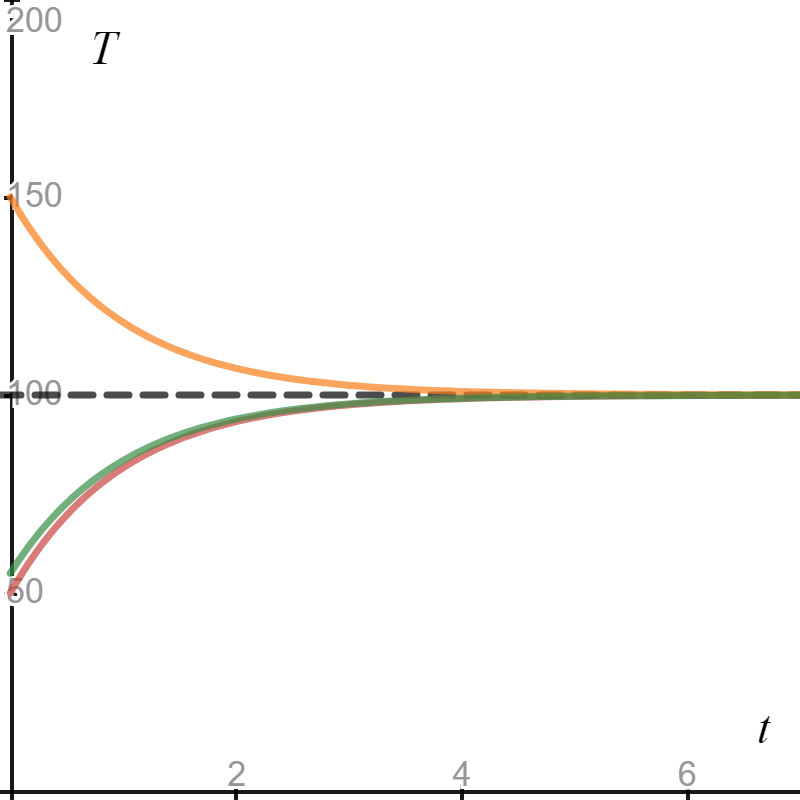
\includegraphics[width=.6\textwidth]{newtons_cooling.png}
    \caption{Black dotted curve is the ambient temperature $T_a=100$. The red curve is the particular solution for $T(0)=50$, the orange curve is the particular solution for $T(0)=150$, and the green curve is the particular solution for $T(0)=55$.}
\end{figure}
Now we can see the temperature of the object approaches the temperature of the ambient environment as time goes on. This is what we expect!
\end{solution}

\newpage

\begin{problem}
    What happens instead if the initial temperature is equal to the ambient temperature? Does your solution reflect this? Does this make physical sense?
\end{problem}
\begin{solution}
If the initial temperature was equal to the ambient temperature then we don't expect the object to change temperature over time.  One would find that we have the equation
\[
100=T(0)=100-e^{-0-C}=100-e^{-C}
\]
and so $e^{-C}=0$ and thus
\[
T(t)=100,
\]
which is what we expect.
\end{solution}

\newpage

\begin{problem}
    Let $\delta = (T_a-T)$. Show that the equation you found in Problem 1 reduces to
    \[
    \delta' = -k\delta.
    \]
    What is this equation describing physically?
\end{problem}
\begin{solution}
Well, note that $\delta'=(T_a-T)'=-T'$.  Thus we can write
\[
\delta'=-T'=-k(T_a-T)=-k\delta.
\]
This equation is describing how the \emph{difference} in temperature of the object versus the ambient environment will change over time. If you were to solve this, you would find that $\delta\to 0$ as $t\to \infty$.
\end{solution}

\newpage

\begin{problem}
    The equation you arrived at earlier, $\delta'(t) = -k\delta(t)$, is \emph{autonomous}.  In this particular instance, it means that this problem has a derivative that is independent of time $t$.  In fact, for this system, this essentially means that total energy is conserved! 
    \begin{enumerate}[(a)]
        \item Using the slope field generator found at: \url{https://www.desmos.com/calculator/p7vd3cdmei}, plot the slope field in the $t\delta$-plane and explore what happens as you vary $k$. What happens when $k=0$? How about $k>0$? How about $k<0$? 
        \item In this slope field plot, explain the symmetry.  Can you see why this shows that we can always choose the initial time to be $t_0=0$ regardless of the value of the initial condition? 
        \item $k$ represents the conductivity of the object.  Explain what the the solutions for $k<0$, $k=0$, and $k>0$ mean physically. Should we think of objects with $k\leq 0$?
        \item If instead we had an equation $y'=-kty$, can you see why we can no longer simply choose $t_0=0$ as the initial time?
    \end{enumerate}
\end{problem}  
\begin{solution}~
\begin{enumerate}[(a)]
    \item Let us plot the slope field for $k=1$, $k=0$, and $k=-1$ to investigate the differences.  
    \begin{figure}[H]
        \centering
        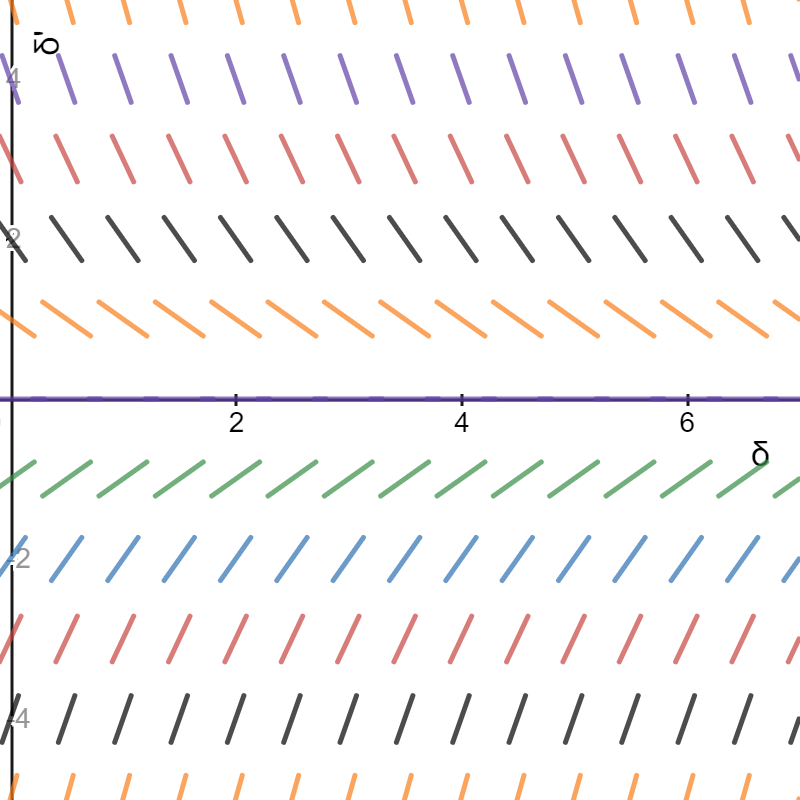
\includegraphics[width=.4\textwidth]{slope_field_k=1.png}
        \caption{The slope field for $k=1$.}
    \end{figure}
    Notice that in this case, we see the slopes are pointing towards the $\delta$-axis. This leads us to the scenario where the difference in temperature will approach zero.\\
    
    \begin{figure}[H]
        \centering
        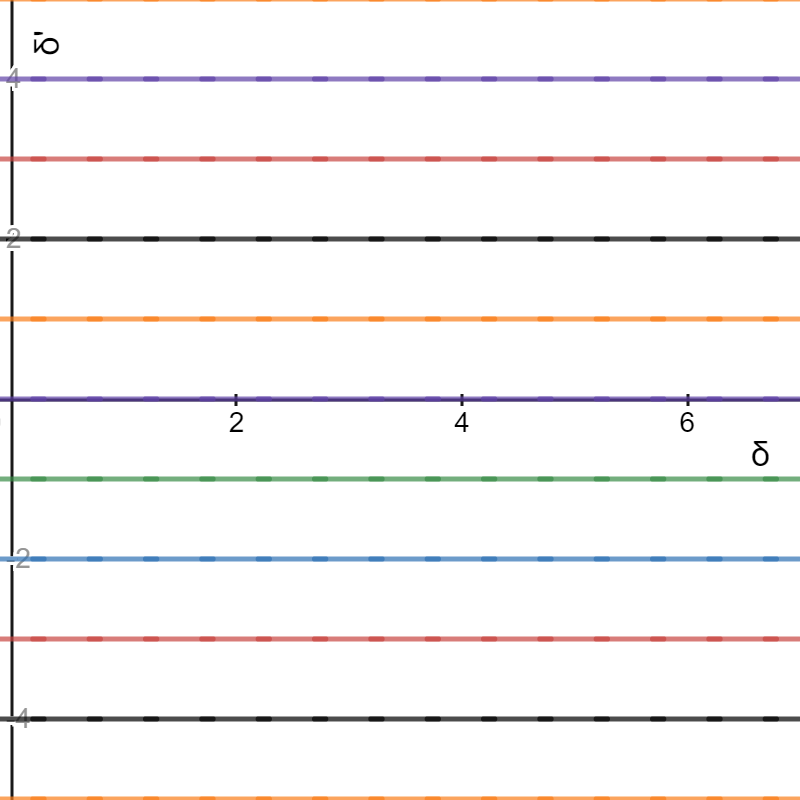
\includegraphics[width=.4\textwidth]{slope_field_k=0.png}
        \caption{The slope field for $k=1$.}
    \end{figure}
    Notice that in this case, we see the slopes are always zero.  Thus, any initial temperature difference in this case will stay the same.  This is not physically what we would expect. So, for the real world Newton cooling problem, we would not allow $k=0$.\\
    
    \begin{figure}[H]
        \centering
        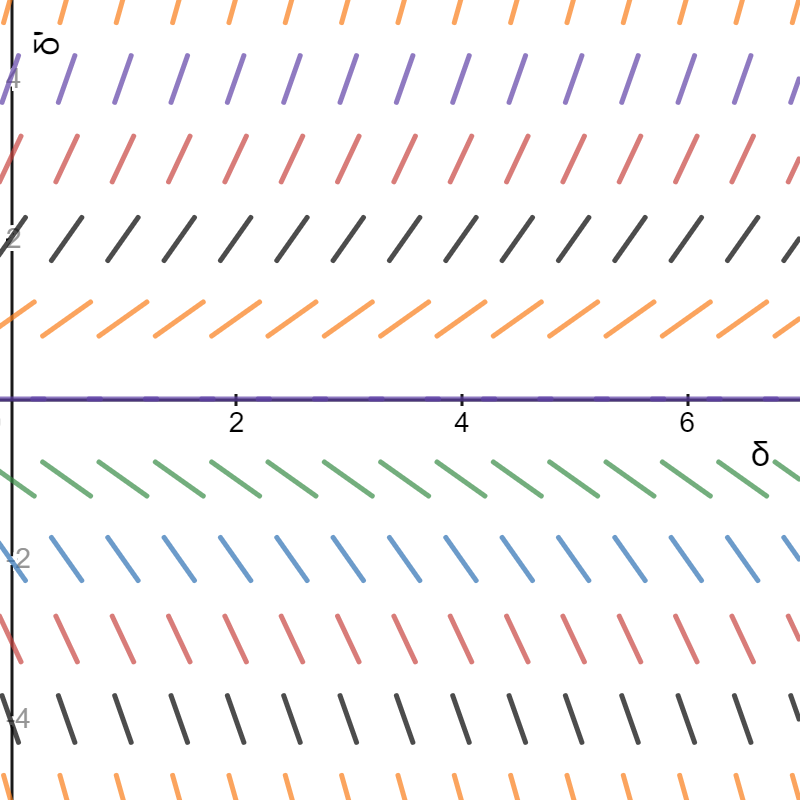
\includegraphics[width=.4\textwidth]{slope_field_k=-1.png}
        \caption{The slope field for $k=1$.}
    \end{figure}
    Notice that in this case, we see the slopes are pointing away from the $\delta$-axis. This leads us to the scenario where the difference in temperature will increase indefinitely. This is also not realistic as this means objects would spontaneously heat up. We thus would rule out $k<0$ in a physical situation.
    
    \item If we look at any given $\delta'$, we notice that if we move in the $\delta$ direction, the slopes remain the same.  This is because of the fact that there is no $t$ itself in the ODE.  So, we have this translational symmetry.  Thus, it does not matter at what time we start making the measurement as the curve will look the same in the end -- it will simply be translated in time.
    
    \item If $k$ represents conductivity, then $k<0$ would represent an object with a negative conductivity. That is, instead of the object radiating heat to the surrounding environment, it would \emph{absorb} heat from the surrounding environment.  This is not typical at all. 
    
    For $k=0$, we have that the object has no conductivity what so ever.  Thus, it will always be the same temperature regardless of the surrounding environment.  This does not happen!
    
    Lastly, for $k>0$, this represents a realistic conductivity.  As was discussed in part (a), we should not consider $k\leq 0$!
    
    \item Let us plot this new equation's slope field for $k>0$.
        \begin{figure}[H]
            \centering
            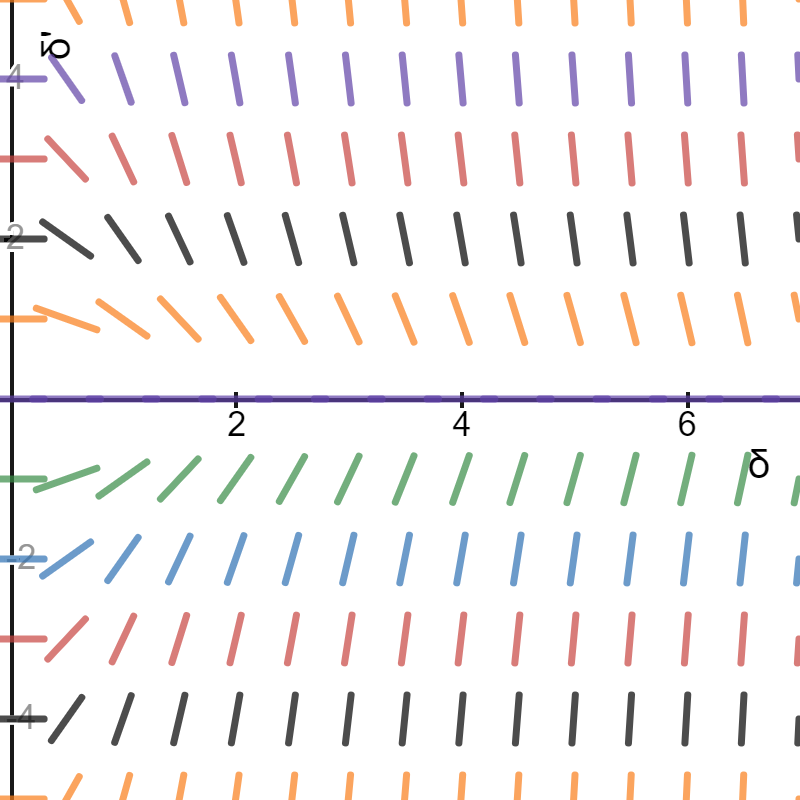
\includegraphics[width=.4\textwidth]{new_slope_field.png}
            \caption{The slope field for $y'=-ty$.}
        \end{figure}
    In this case, we no longer have the same symmetry as we saw before.  Indeed, we can note that the derivative of our solution depends on time explicitly (since $t$ appears in the ODE). This means that the time in which we start making measurements \emph{does} matter in this case! This may represent cooling of an object that we are also applying heat to as we increase time.
\end{enumerate}
\end{solution}

\newpage

\begin{center}
    Problems 7-8 are related.
\end{center}
\begin{problem}
    Show that $x=c_1\sin(t)+c_2\cos(t)$ is a general solution to the equation
    \[
        x''+x=0.
    \]
\end{problem}
\begin{solution}
We plug in our guess for $x$ into the left hand side of the equation and we'll check to see that we get zero.  So,
\begin{align*}
    x''+x&=(c_1\sin(t)+c_2\cos(t))''+(c_1\sin(t)+c_2\cos(t))\\
    &= -c_1\sin(t)-c_2\cos(t)+c_1\sin(t)+c_2\cos(t)\\
    &=0.
\end{align*}
Indeed, this $x$ does solve our equation.
\end{solution}

\newpage

\begin{problem}
    Find the particular solution if $x(0)=1$ and $x'(0)=0$. Plot your solution in the $t,x$-plane and in the $x,x'$-plane. 
\end{problem}
\begin{solution}
Now, we use our initial data with our general solution above
\begin{align*}
    1=x(0)=c_1\sin(0)+c_2\cos(0)=c_2
\end{align*}
so $c_2=1$.  Also, we have
\[
0=x'(0)=c_1\cos(0)-\sin(0)=c_1
\]
so $c_1=0$. Thus, our particular solution is
\[
\boxed{x(t) = \cos(t).}
\]

We can then plot this solution in the $tx$-plane,
\begin{figure}[H]
    \centering 
    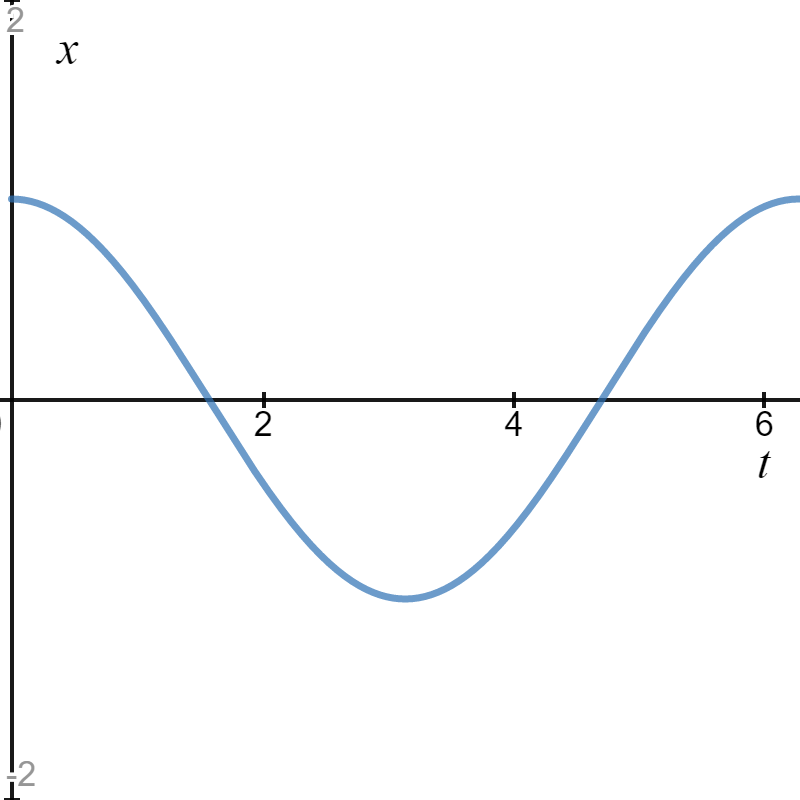
\includegraphics[width=.5\textwidth]{tx_solution.png}
    \caption{The particular solution $x(t)=\cos(t)$ plotted in the $xx'$-plane for $t\in [0,2\pi]$.}
\end{figure}
and in the $xx'$-plane.
\begin{figure}[H]
    \centering 
    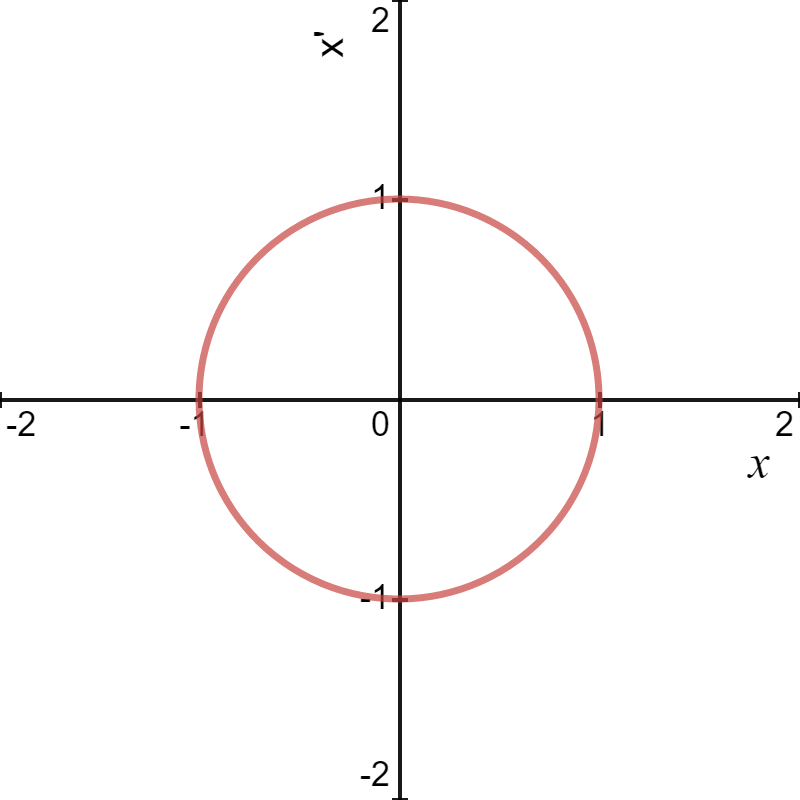
\includegraphics[width=.5\textwidth]{x_xprime_solution.png}
    \caption{The particular solution $x(t)=\cos(t)$ plotted in the $tx$-plane for $t\in [0,2\pi]$.}
\end{figure}
\end{solution}

\newpage

\begin{problem}
    Consider the differential equation
    \[
    x'=\frac{x^2+tx+t^2}{tx}.
    \]
    \begin{enumerate}[(a)]
        \item Let $f(x,t)=\frac{x^2+tx+t^2}{tx}$.  Show that $f(\lambda x, \lambda t)=f(x,t)$.
        \item Use the substitution $u=\frac{x}{t}$ in order to make the original equation separable.
        \item Find the general solution to this separable equation in terms of $u$ and $t$. You may use Wolfram Alpha to compute the necessary integral.
        \item Find the solution to the original equation using the substitution $u=\frac{x}{t}$ and your solution from (c).
    \end{enumerate}
\end{problem}
\begin{solution}~
\begin{enumerate}[(a)]
    \item Take
    \begin{align*}
        f(\lambda x, \lambda t) &= \frac{(\lambda x)^2 + (\lambda t)(\lambda x) + (\lambda t)^2}{(\lambda t) (\lambda x)}\\
        &= \frac{\lambda^2 x^2 + \lambda^2 tx + \lambda^2 t^2}{\lambda^2 tx}\\
        &= \frac{x^2+tx+t^2}{tx}.
    \end{align*}
    Indeed we have that $f(\lambda x, \lambda t)=f(x,t)$.
    \item Now we let $u=\frac{x}{t}$ and we can note that this yields
    \[
    x' = tu' + u.
    \]
    Thus, we have
    \begin{align*}
        tu'+u &= \frac{x^2}{tx} + \frac{tx}{tx} + \frac{t^2}{tx}\\
        &= \frac{x}{t} + 1 + \frac{t}{x}\\
        &= u + 1 + \frac{1}{u}.
    \end{align*}
    It follows that we then have
    \[
        u' = \frac{1}{t}\left(1+\frac{1}{u}\right),
    \]
    which is separable.
    
\item We can write
\[
1+\frac{1}{u} = \frac{u+1}{u}
\]
and separate to get
\[
\frac{u}{u+1} du = \frac{1}{t}dt.
\]
Then, integrating yields
\[
u-\ln(u+1) = \ln(t) + C,
\]
which cannot be simplified more (unless we introduce new functions).
\item Noting that $u=\frac{x}{t}$, we have
\[
\frac{x}{t} - \ln\left(\frac{x}{t} + 1\right) = \ln(t)+C.
\]
\end{enumerate}
\end{solution}


\end{document}
